\section{Accelerator and Beamline}
The Thomas Jefferson National Accelerator Facility (JLab), located in
Newport News, VA, is home to the Continuous Electron Beam Accelerator Facility
(CEBAF) which delivers a stable, high energy, high duty factor electron beam
to four experimental halls.
The data for the E12-06-107 experiment were taken in early 2018 in Hall C at
JLab.

\begin{figure}[ht]
    \centering
    \begin{subfigure}[b]{0.9\textwidth}
        \centering
        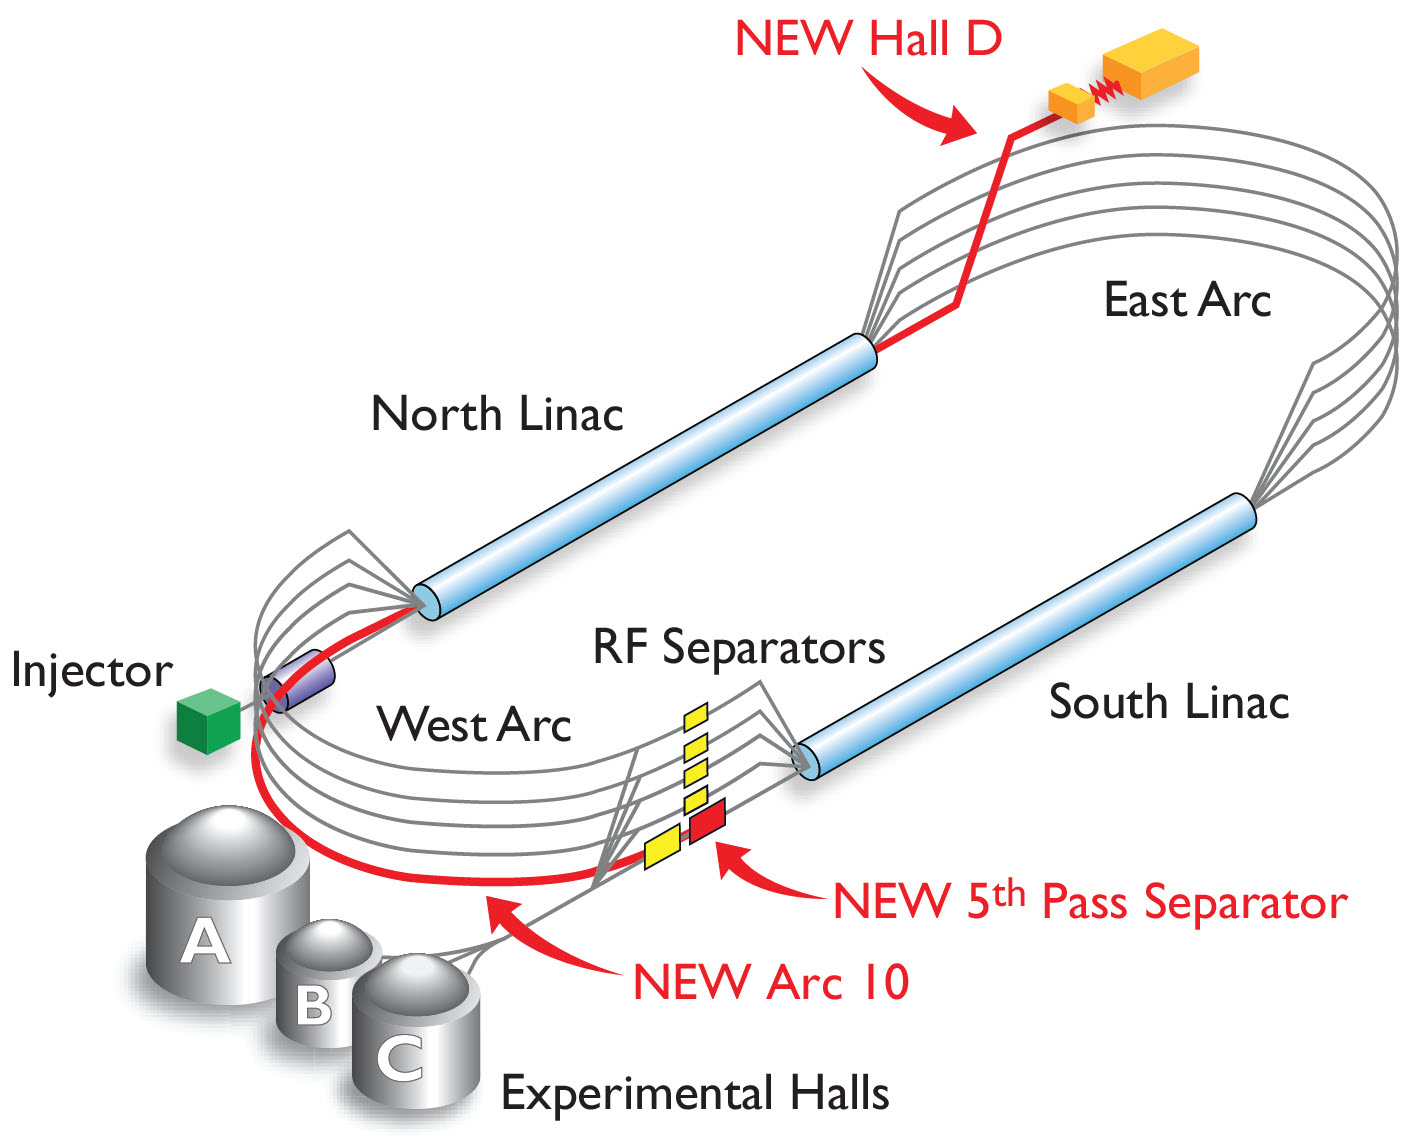
\includegraphics[height=8cm]{chap3/CEBAF_cartoon.jpg}
        \caption{A schematic view of the CEBAF accelerator.}
        \label{fig:CEBAF_cartoon}
    \end{subfigure}
    \vspace{0.1cm}
    \\
    \begin{subfigure}[b]{0.9\textwidth}
        \centering
        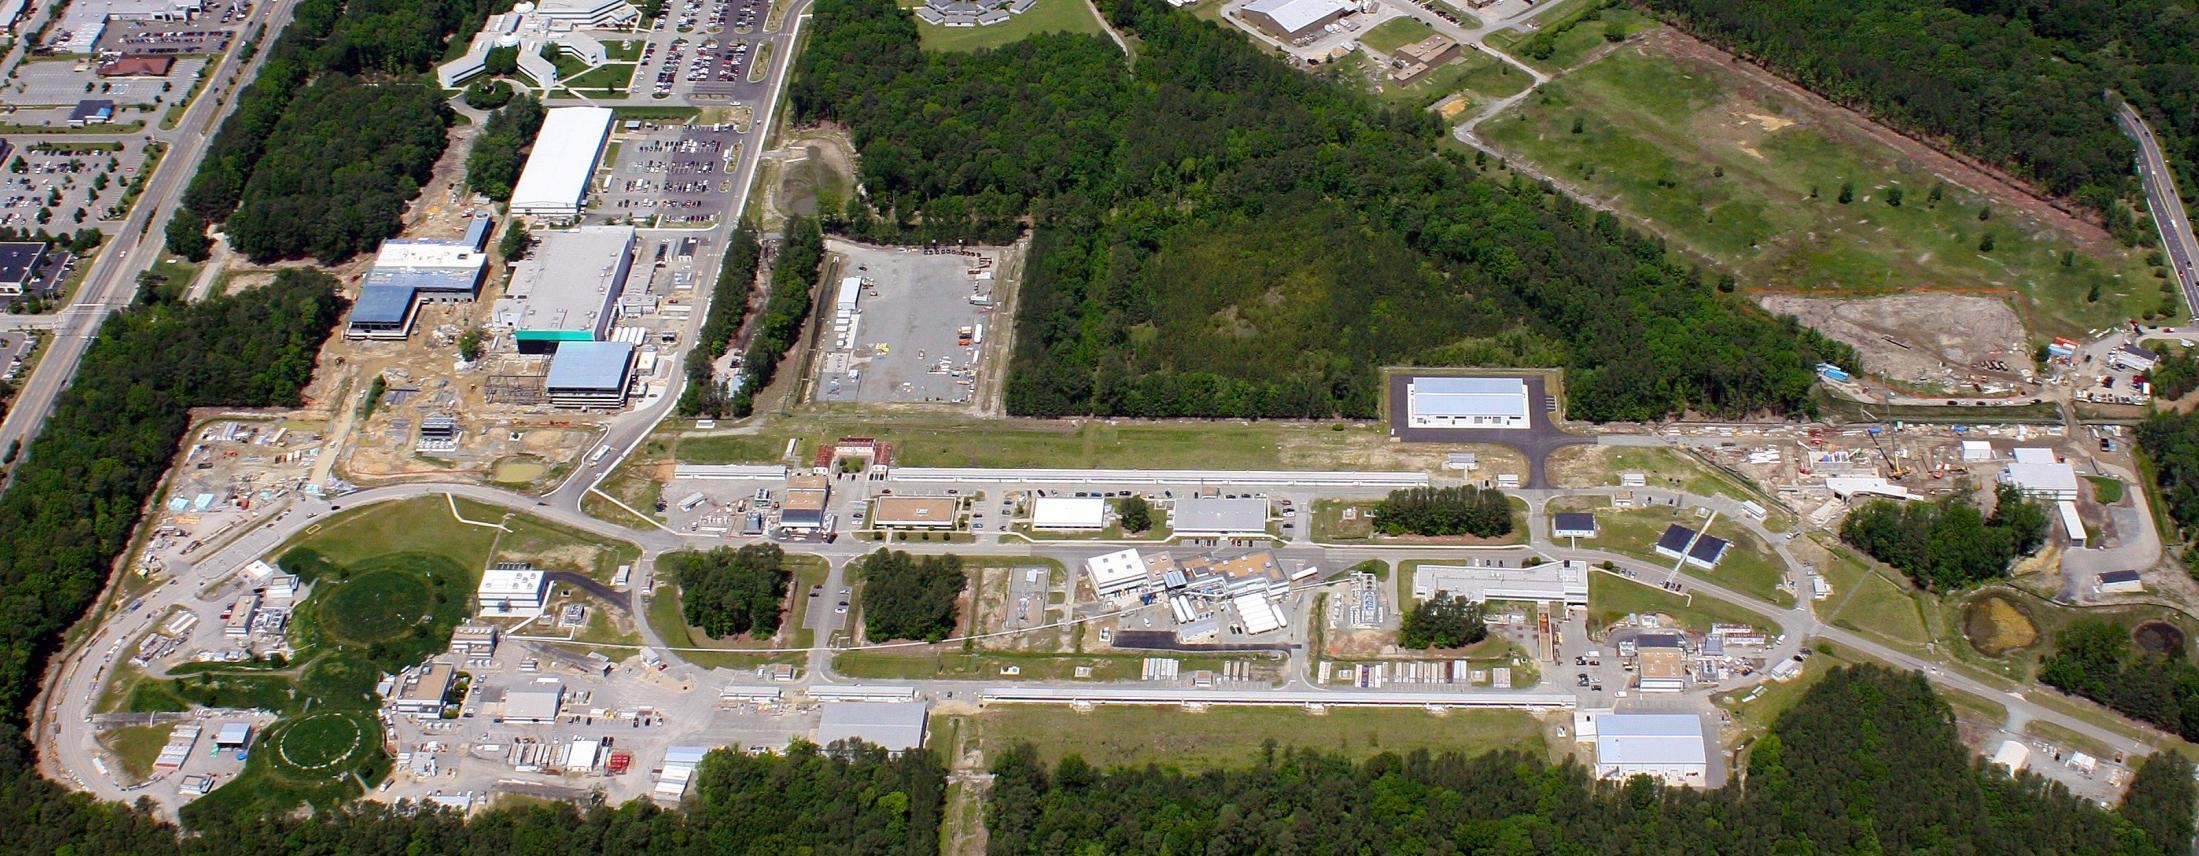
\includegraphics[width=\textwidth]{chap3/CEBAF_aerial_horizontal.jpg}
        \caption{An aerial photograph of the CEBAF accelerator site.}
        \label{fig:CEBAF_aerial}
    \end{subfigure}
    \caption{The Continuous Electron Beam Accelerator Facility}
    \label{fig:CEBAF}
\end{figure}


\subsection{CEBAF}
CEBAF consists of an injector that generates a beam of \SI{123}{MeV} electrons,
a racetrack-shaped combination of linear accelerators (linacs) and
recirculation arcs, and extraction regions.


The injector consists of a \SI{130}{keV} electron gun, a bunching
system\footnote{The prebuncher, chopper, and buncher separate the continuous
beam into ``bunches'' of electrons that can be independently removed from the
recirculating beam using radiofrequency (RF) separators, allowing simultaneous
beam delivery to all four experimental halls.~\cite{Kazimi_2019}}, and
superconducting radiofrequency linacs that accelerate electrons to
an energy of \SI{123}{MeV} before they enter the accelerator ring.


The accelerator ring consists of two linacs, each of which gives
the beam an additional \SI{1.1}{GeV} per pass.
At the end of each linac, the beam can be extracted and delivered to an
experimental hall, or sent back to be recirculated and accelerated to a maximum
of \SI{10.9}{GeV} for Halls A, B, and C or \SI{12}{GeV} for Hall D.


Because the beam in the linacs contains bunches with different energies,
different magnetic field strengths are necessary in the recirculation arcs.
Dipole magnets are used to spread the beam vertically into separate arcs
(consisting of bending dipoles and focusing quadrupoles)
tuned to different pass energies, and then recombine them for extraction to
experimental halls or additional passes through the linacs.


\begin{figure}[!h]
    \centering
    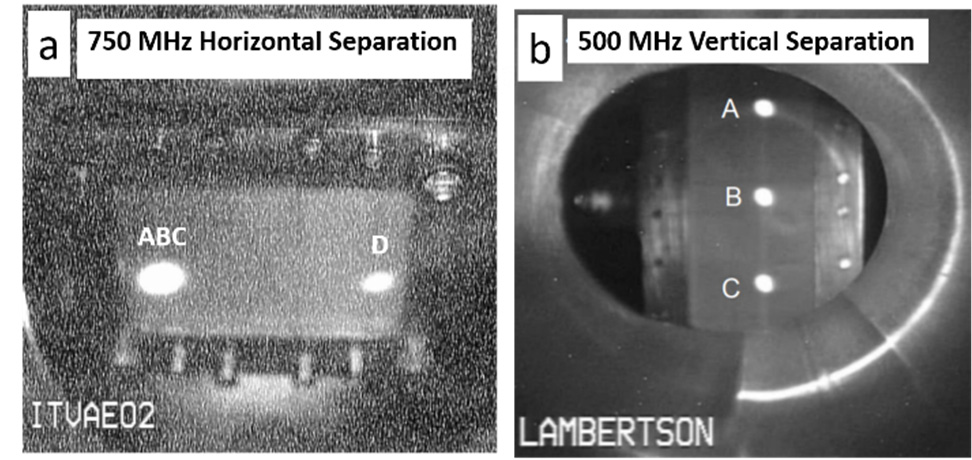
\includegraphics[width=0.7\textwidth]{chap3/RF_separation.jpg}
    \caption{(a) Beam viewer downstream from 5th pass \SI{748.5}{MHz} RF
             separator showing horizontal separation of Hall D's beam.
             (b) Beam view downstream from the \SI{499}{MHz} RF separator
             showing vertical separation of the beams to be delivered to Halls
             A, B, and C.
             }
    \label{fig:RF_separation}
\end{figure}


The injector's buncher system creates a beam that has a high duty factor but
also has an internal structure consisting of \SI{2}{ps} long bunches of
electrons that come at a rate of \SI{1497}{MHz}.
RF cavities with a fundamental frequency of \SI{499}{MHz} (or \SI{748.5}{MHz}
for Hall D) separate these bunches spatially to allow them to be separated from
the beam and delivered to the halls independently.
This results in beam bunches that arrive at the target every \SI{2}{ns}.

\subsection{Hall C Arc and Beamline}
Once separated from recirculation through the accelerator ring, the beam passes
through the Hall C arc and beamline.
Along the way the beam passes though several diagnostic elements including
superharps, beam position monitors (BCMs), beam current monitors (BCMs), and
polarimeters.

%TODO: Find a diagram of the arc and beamline that isn't "too" cluttered.

\subsubsection{Superharps}
\begin{figure}[!h]
    \centering
    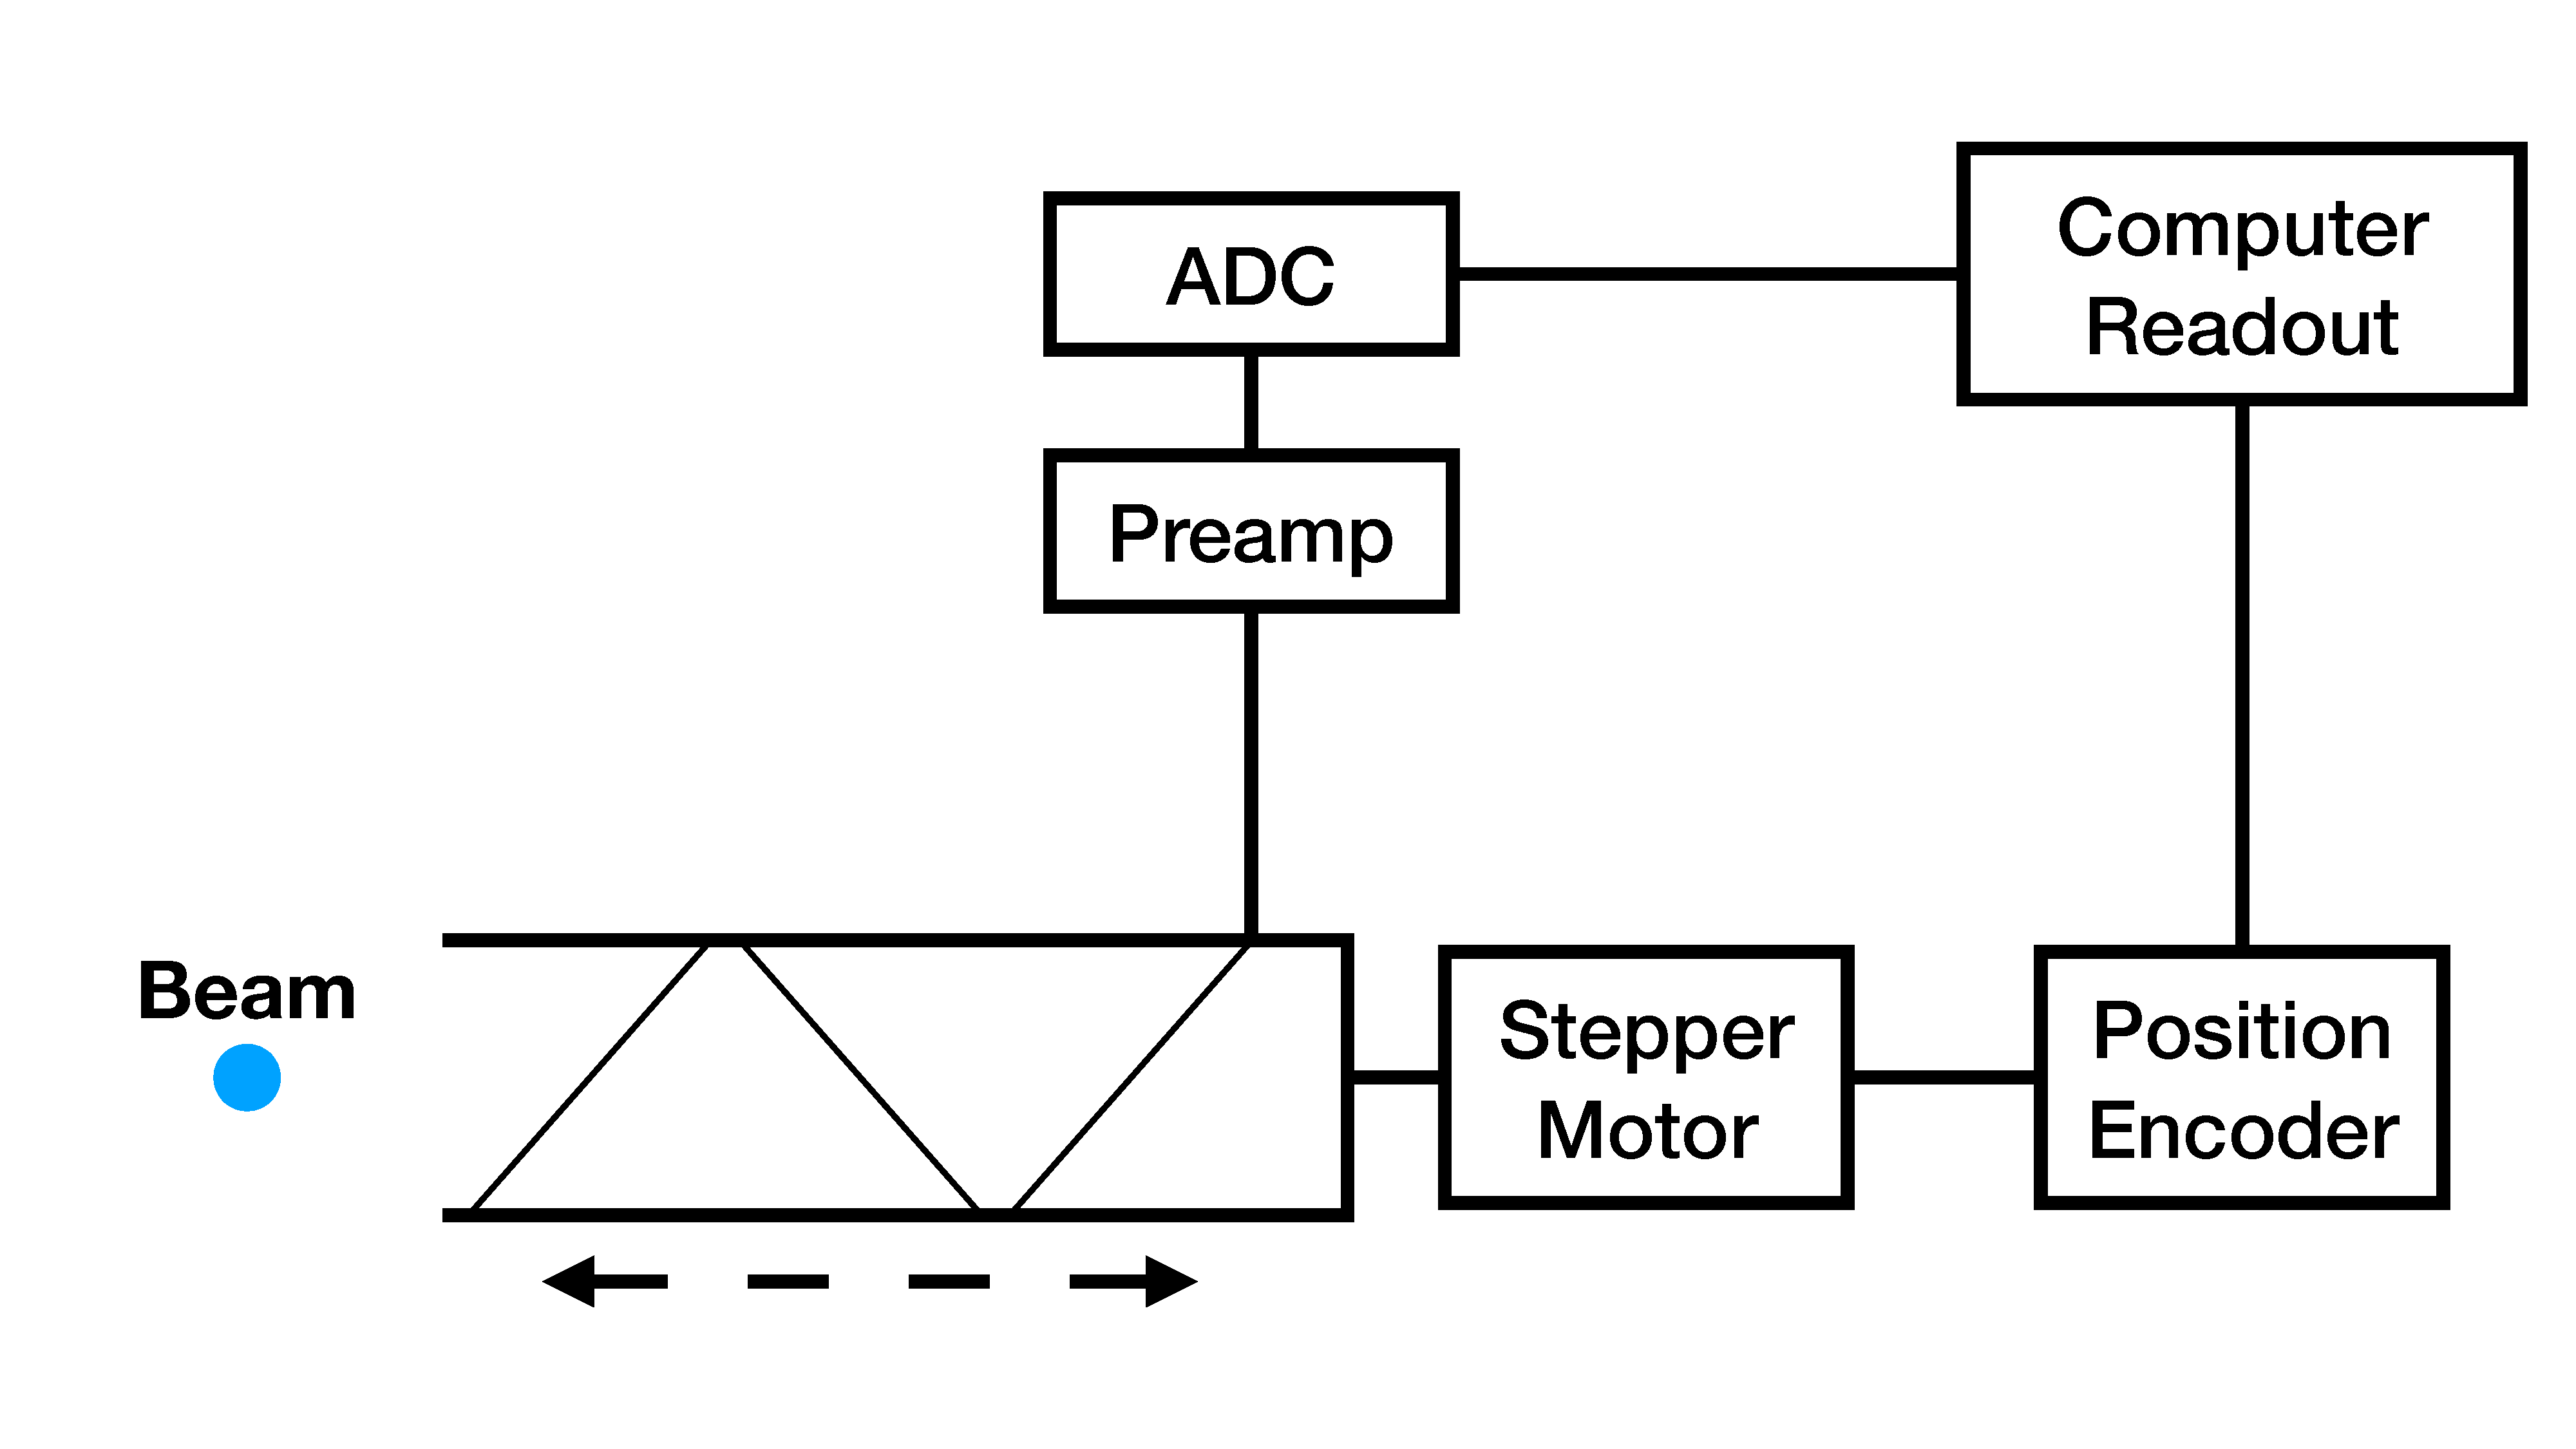
\includegraphics[width=0.7\textwidth]{chap3/Superharp_diagram.pdf}
    \caption{Schematic representation of a superharp. The motor moves the fork
             into the beam, where beam electrons interact with the wires,
             creating a signal registered by the ADC.}
    \label{fig:superharp_diagram}
\end{figure}
\begin{figure}[!h]
    \centering
    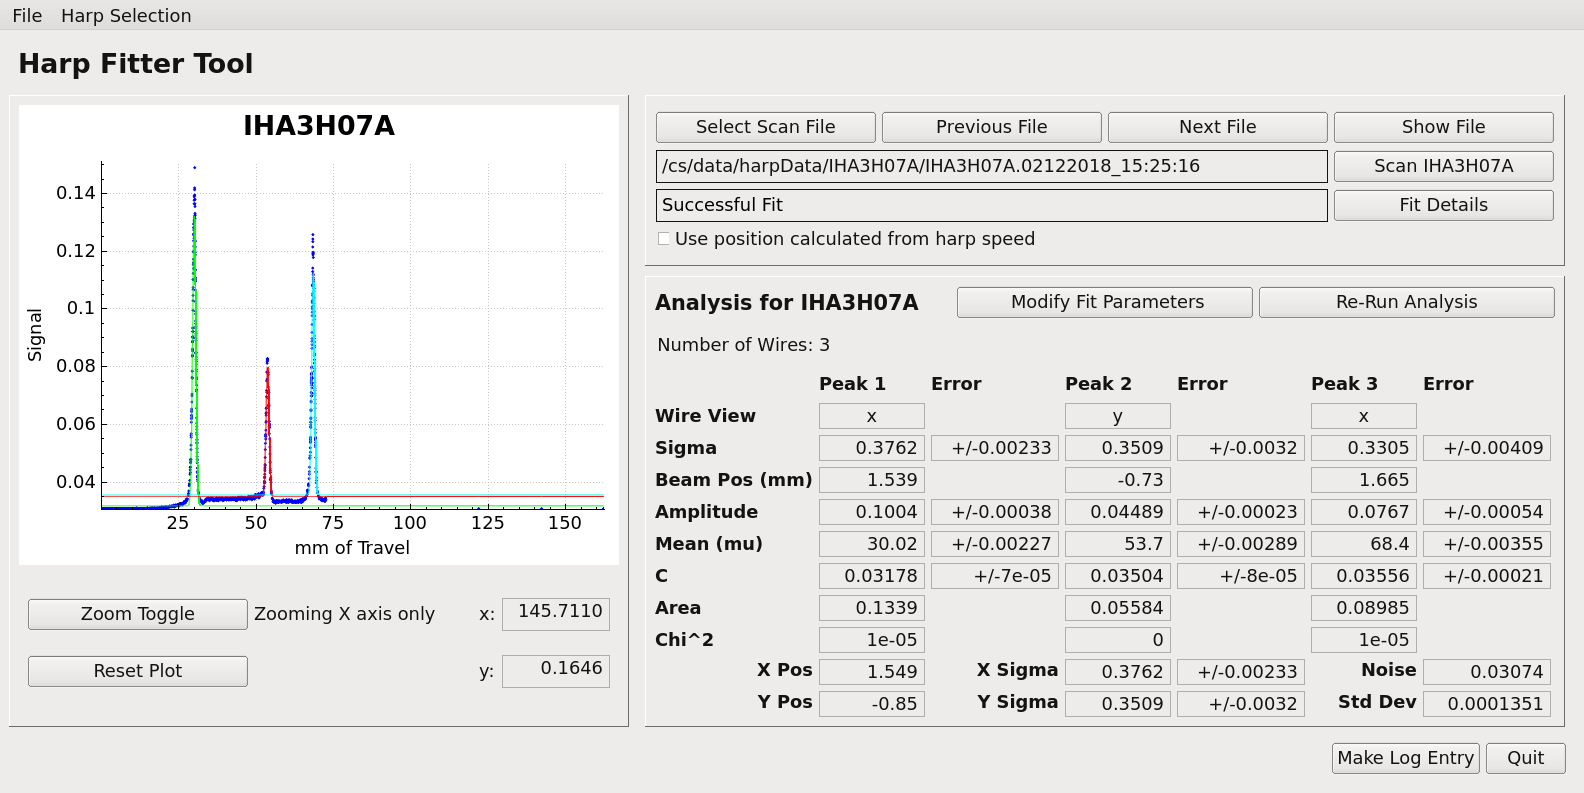
\includegraphics[width=1.0\textwidth]{chap3/harpFitter.png}
    \caption{The Harp Fitter GUI, which fits the signal from a superharp and
             reports the estimated beam position and width.
            }
    \label{fig:harp_fitter}
\end{figure}

Superharps~\cite{Yan_1995} are used to measure the beam's position, $XY$
profile, and energy.
They also provide information to the Compton and M\o{}ller polarimeters.


Each superharp consists of a fork with two vertical wires and one horizontal
wire, attached to a stepper motor that allows it to be inserted and removed
from the beam.
A position encoder measures the position of the fork.
As the wires pass through the beam, secondary electron emission creates a
current in the wires, yielding a signal that can be read out by an
analog-to-digital converter (ADC).
The profile of the beam can be estimated by fitting the wire signals
vs encoder position, as shown in~\ref{fig:harp_fitter}.


\subsubsection{Beam Position Monitors}
Three BPMs (IPM3H07A, IPM3H07B, IPM3H07C) upstream from the target provide
measurements of the relative beam position within \SI{100}{\micro\meter}.
The BPMs' absolute position can be calibrated with respect to the adjacent
superharps, IHA3H07A and IHA3H07B.


Each BPM consists of four antennae attached to a cylindrical cavity that froms
part of the beamline enclosure.
Two pairs of antannae are located opposite each other, with each pair \ang{90}
from the other, forming an X'Y' coordinate system rotated \ang{45} from the
X and Y axes of the EPICS (left-handed) coordinate system.
The beam induces a signal in each antenna, which is tuned to \SI{499}{Hz}
(a subharmonic of the beam).
The amplitude of this signal is inversely proportional to the distance from the
beam to the antenna, so the relative distance can be computed by taking the
ratio of the difference to the sum of the signals from pairs of antennae on
opposite sides of the enclosure.


Superharp measurements of the beam position are invasive and cannot be taken
during production data acquisition.
BPM measurements are noninvasive and can be taken continuously.
Each BPM measurement is averaged over \SI{0.3}{s} and logged by EPICS every
\SI{1}{s}.
The BPMs' raw outputs are also recorded for every event in the CODA datastream.
Converting these raw values to physical outputs requires calibrating the
parallel electronics chain to the EPICS data.

\subsubsection{Beam Current Monitors}
The system for monitoring beam current consists of several resonant-cavity BCMs
and one parametric-curent-transformer Unser monitor.


The Unser current monitor~\cite{Unser_1991} consists of a toroidal pickup
placed around the beam pipe.
The beam's magnetic field induces a flux in the toroid, which a feedback system
tries to cancel by driving a current through a compensating coil.
This compensating current is proportional to the beam current.


The BCMs consist of high Q ($\sim 500$) stainless steel cylindrical waveguides
tuned to the fundamental frequency of the beam.
The voltage at their output is proportional to the beam current.


The gain of the Unser is a relatively stable
\SI{4}{\milli\volt\per\micro\ampere} but has an unstable offset that is known
to drift significantly on a time scale of
minutes~\cite{Standard_Equipment_Manual}.
This offset can be corrected for by intermittently taking calibration runs with
no current.
The Unser's gain can be precisely measured during downtime by passing a known
DC current through it during downtime.
The gains of the BCMs are unstable and must be calibrated relative to the
Unser's.
In contrast to the Unser, the BCMs have a relatively stable offset.


The output of both the Unser and BCMs\footnote{The BCMs' RF outputs must first
be sent through an analog (for BCM1 and BCM2) or digital (for BCM4A, BCM4B, and
BCM4C) downconverter.} are sent to voltage-to-frequency converters whose ouputs
are sent to DAQ scalers as well as a VME crate for processing and integration
into the EPICS stream.

\subsubsection{Beam Rastering System}
To prevent overheating and damage to solid targets and local boiling in
cryogenic targets, Hall C uses a ``fast raster'' system~\cite{Yan_2005}.
The system consists of two sets horizontal and vertical steering magnets
that rapidly vary the beam position.
The magnets consist of bedstead air-core windings of Litz\footnote{``Litz is a
short term used for a German word ‘Litzendraht’ that means braided wire. Litz
cable consists of multiple strands and each strand is coated by insulation
film. The entire cable is also subdivided into several twisted groups, which
are formed by twisted basic strands. The major purpose for use of the Litz
cable is to reduce power loss caused by the Eddy current.''~\cite{Yan_2005}}
cables.
The raster magnets are located about \SI{20}{\meter} upstream from the center
of the target chamber, a region that does not include any optical focusing
elements so as decouple the raster system from beam optics tuning.
The final profile of the rastered beam on the target will be a result of a
combination of the beam optics and raster magnets.


Hall C used a Lissajous raster system, driven by sinusoidal magnet currents,
from 1996 to 2002 that slowed down at the edges of the raster scan.
This resulted in the rastered beam spending more time at the edges and corners
than the central region of the raster scan.
To more evenly distribute the raster scan, the fast raster system now uses a
\SI{25}{\kilo\Hz} triangle wave to drive the raster magnets.

\begin{figure}[h]
    \centering
    \begin{subfigure}[b]{0.4\textwidth}
        \centering
        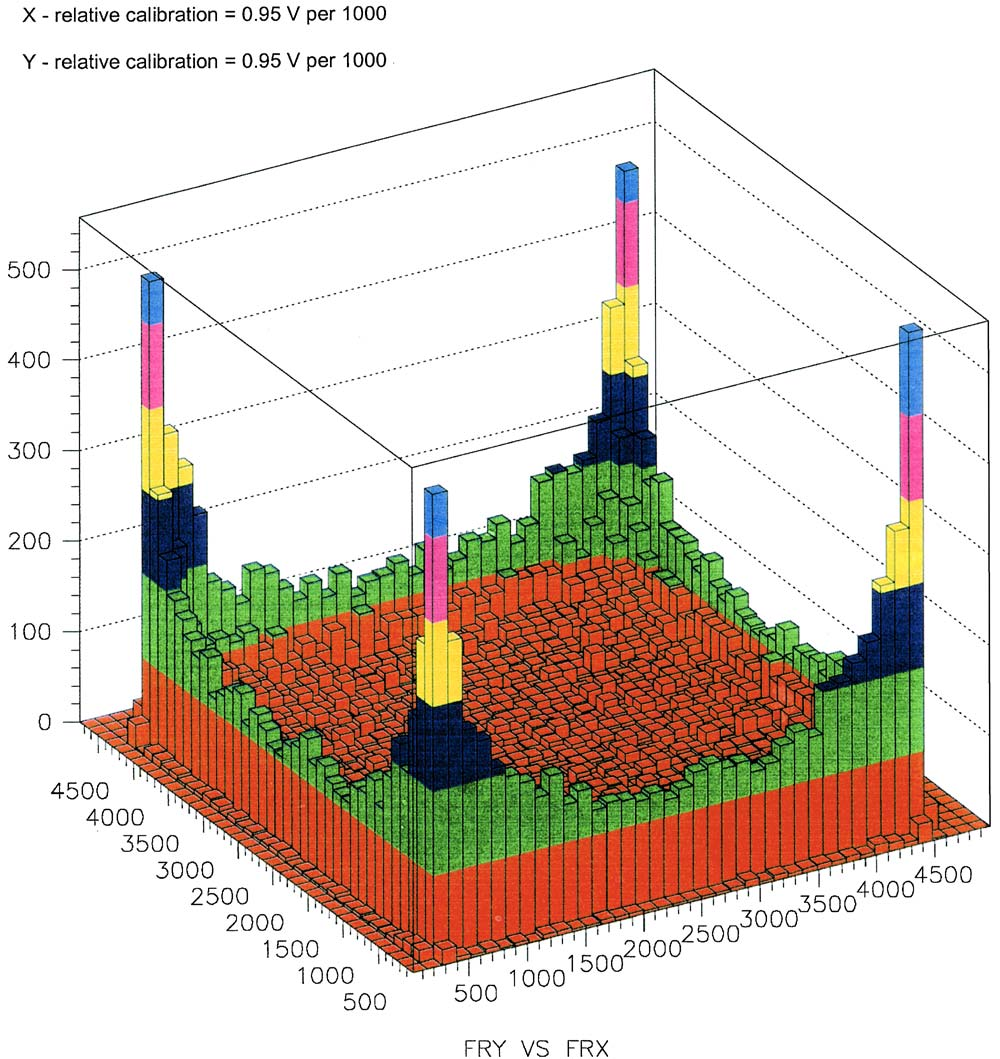
\includegraphics[width=\textwidth]{chap3/Lissajous_raster_colz.jpg}
        \caption{Old Lissajous raster pattern.}
        \label{fig:Lissajous_raster}
    \end{subfigure}
    \hfill
    \begin{subfigure}[b]{0.4\textwidth}
        \centering
        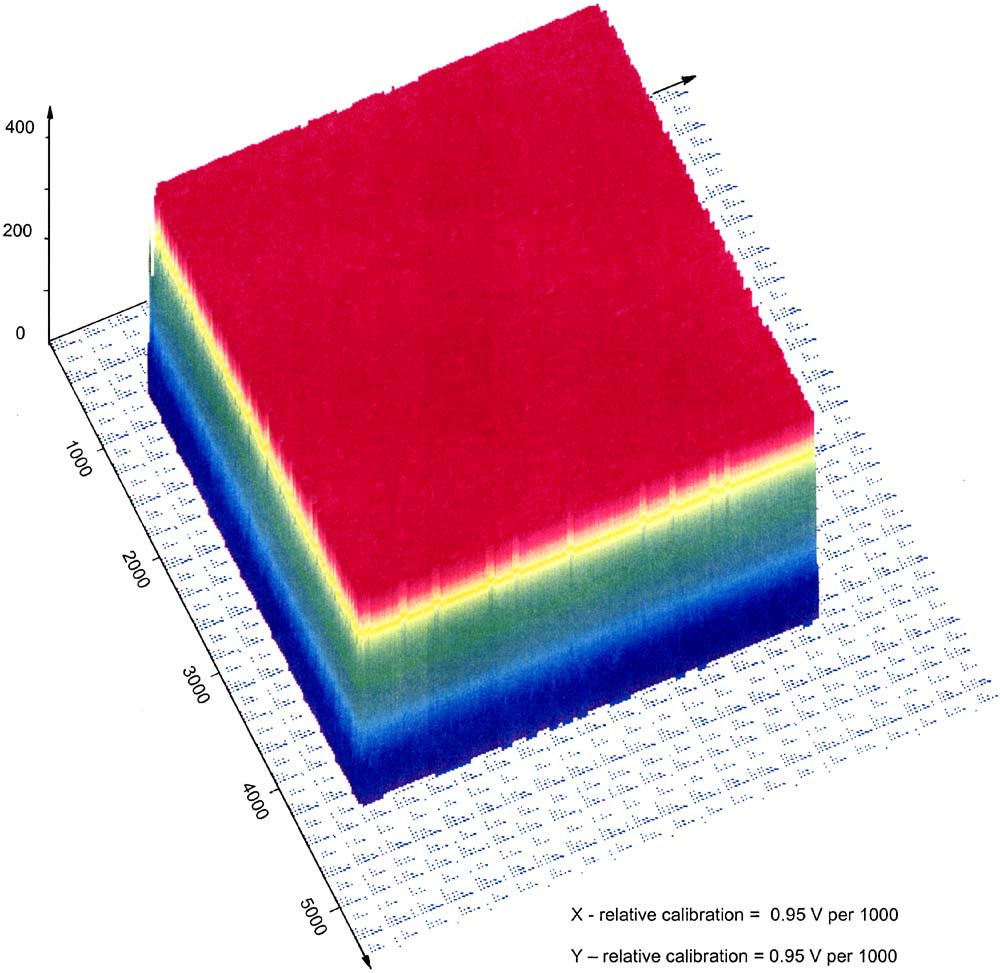
\includegraphics[width=\textwidth]{chap3/triangle_raster_colz.jpg}
        \caption{New triangle raster pattern.}
        \label{fig:triangle_raster}
    \end{subfigure}
    \caption{A comparison of the distributions of the x and y positions of the
             beam on target for data taken with the old and new (i.e. in
             operation since 2002) raster patterns. Figure reproduced
             from~\cite{Yan_2005}.}
    \label{fig:raster_comparison}
\end{figure}

% NOTE: We used a 2x2 cm^2 raster.
% In some of the luminosity scan runs I noticed some peaks on the edges of the
% raster scans. BUT those might be for larger raster sizes.
% Should compare voltage vs cm
